\chapter{Bundle Adjustment}

Bundle adjustment is the process of simultaneously adjusting the
properties of multiple cameras and the 3D locations of the objects
they see, to minimize the error between the estimated forward
projection of the 3D objects and their measured location in the captured
images. 

\begin{figure}[htp]
  \begin{center}
  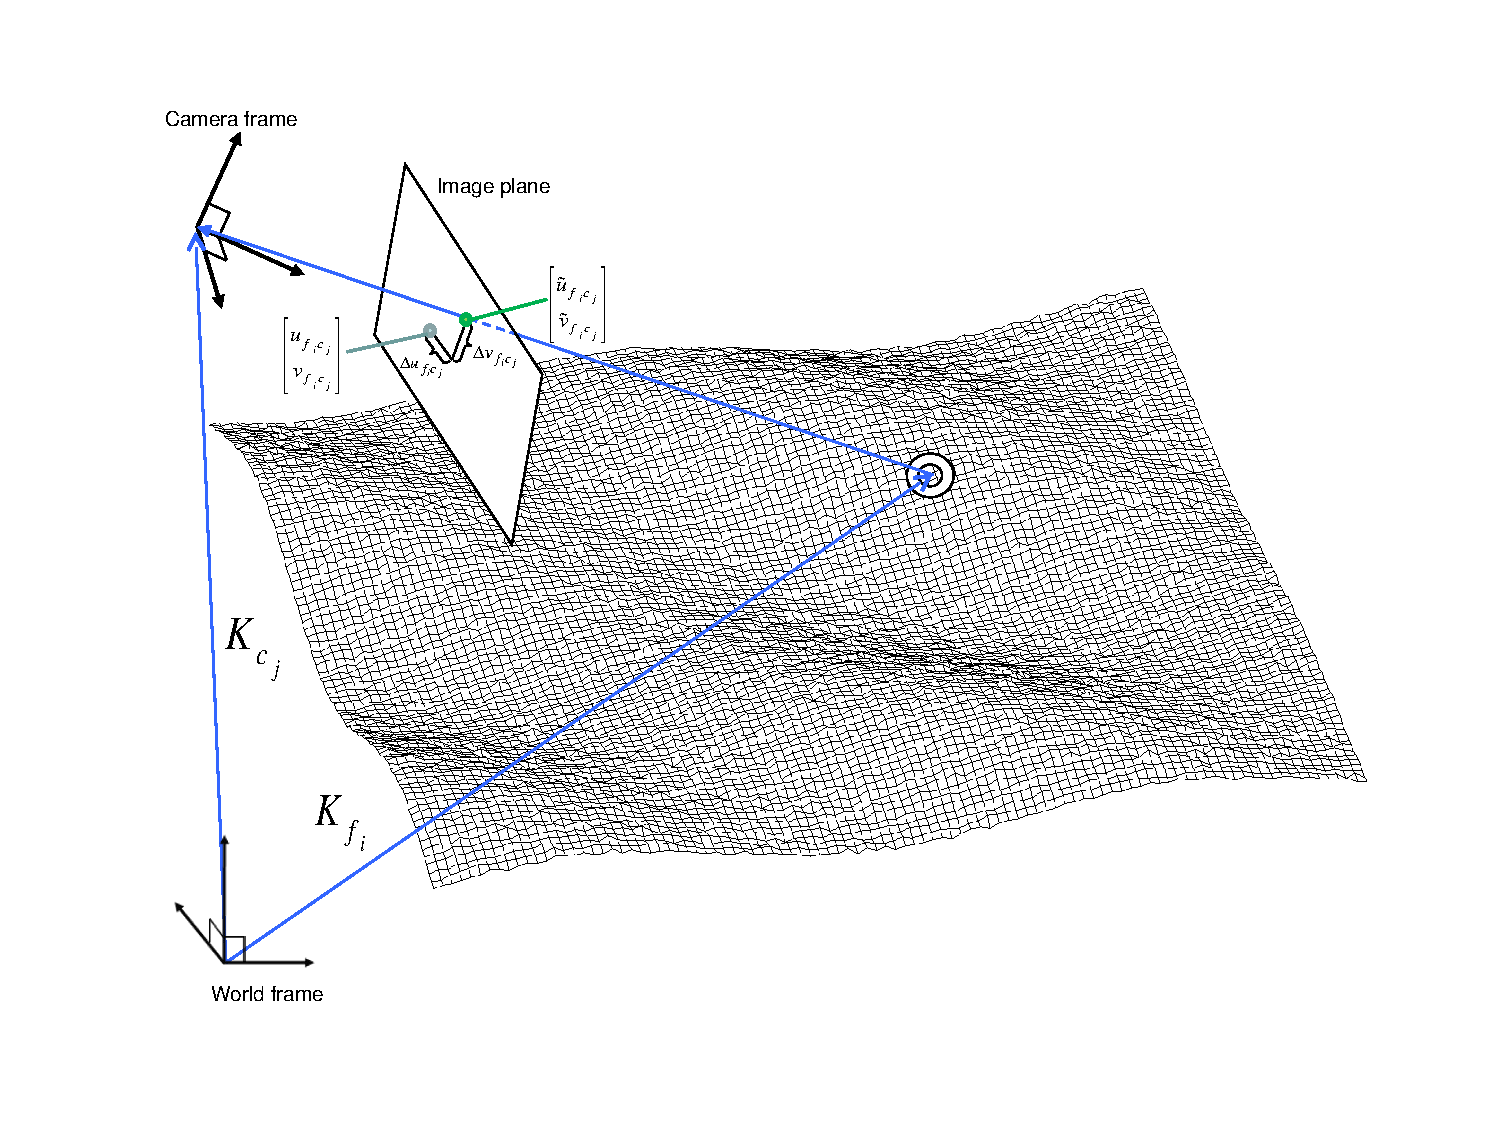
\includegraphics[trim=20mm 20mm 20mm 15mm,clip,width=6in]{images/ba_feature_observation.pdf}
  \end{center}
  \caption{ A feature observation in Bundle Adjustment. \cite{moore09} }
  \label{fig:ba_feature}
\end{figure}

This has application as an optional step between the capture
of images and the creation of DEMs. There is always an amount of error
with the recorded position and orientation of cameras and Bundle
Adjustment can be used to refine these measurements. This will allow
DEMs from multiple cameras to align better with one another. Bundle
Adjustment can also take advantage of Ground Control Points (GCPs),
which are accurately measured 3D locations on the surface of the DEM. GCPs
can be used to improve the alignment of the DEMs or align the new DEM
to a past data product. Finally, even though Bundle Adjustment
calculates the location of the 3D objects it views, only the final
properties of cameras are recorded in the Ames Stereo Pipeline. Those
properties are loaded into \texttt{stereo} which will then use it's own
method for triangulation.

\subsection{A deeper understanding}

Bundle Adjustment in Ames Stereo Pipeline revolves around the
Levenberg-Marquardt Algorithm (LMA) which is a method for minimizing a
function. In the case of Bundle Adjustment, the error $\epsilon$ is
the pixel difference between an objects location in an image,
$[u_{f},v_{f}]$, and it's forward projection through the camera,
$[\tilde{u}_{f},\tilde{v}_{f}]$. The goal is to solve for an update to
the parameters of the cameras and point positions, apply them, and
then repeat until the update supplied by LMA goes to zero. The
equation for LMA is below:

\begin{equation}
\mbox{\boldmath$\delta$} = \frac{\mbox{\boldmath$J^T\epsilon$}}{\bf{J^TJ}+\lambda\bf{I}}
\label{eqn: Levenberg-Marquardt Algorithm}
\end{equation}

LMA is a hybrid of two minimization techniques, gauss-newton and
gradient decent. Where the control between these two methods is the
parameter $\lambda$ which will change in value during the process of
Bundle Adjustment. A high value of $\lambda$ forces LMA to act like
gradient decent, and is what will happen at the beginning of bundle
adjustment when the camera parameters are far away from their final
solution. A low value of $\lambda$ drives LMA into the gauss-newton
method; at which it will take small steps in updating the camera
values. When Bundle Adjustment is almost finished and is close to the
solution, it will lower $\lambda$.

Since Bundle Adjustment is an iterative method, it would be happy to
keep processing new updates to camera parameters all day. To avoid
this, there are several shut-off conditions. The first is when the
update {\boldmath$\delta$} becomes insignificantly small. The second
is when the error measurement, {\boldmath$\epsilon$}, becomes
insignificantly small. Both of these conditions' thresholds are
defined within the bundle adjuster's code and is not allowed for the
user to change. The final shut off condition is when the number of
iterations becomes too large. It is important to understand that when
this shut off condition happens, bundle adjustment has not finished
refining the parameters of the cameras but they are a step closer to
the solution. The maximum number of iterations is changeable by the
user so they can decide how much time they're will to dedicate to the
correction of the data. The number of iterations Bundle Adjustment
takes to converge on the solution can be anywhere between 20
iterations to several hundred.

If you are interested in more information on the math of Bundle
Adjustment and the arrangement of the problem, we recommend reading
Appendix 6 in the {\em Multiple View Geometry} \cite{hartley04}.
For more information on why LMA is used instead of the many other
optimization algorithms, try reading {\em Bundle Adjustment – A Modern
Synthesis} \cite{triggs00}.

\section{ISIS Adjust}

Purpose, Bundle Adjustment Model, Supported Equations, Examples

\subsection{Options}

\begin{verbatim}
--cnet, -c [control network file]
\end{verbatim}

\emph{Optional.} Feeding this option will force ISIS Adjust to use an
already built control network. If not fed, ISIS Adjust will look for
match files in current operating directory with names similar to the
input images to build it's control network from. If
\texttt{isis\_adjust} creates it's own control network file, it will
save it as \verb=isis_adjust.cnet=.

\begin{verbatim}
--lambda, -l [value]
\end{verbatim}

\emph{Optional.} This set the starting value for $\lambda$. Bundle
Adjustment will naturally select a value for $\lambda$ it thinks is
best for the starting error, but this argument can be used to override
that. \emph{It's not recommended to change the starting value of
  $\lambda$ except for experienced users.}

\begin{verbatim}
--position-sigma [default = 100]
\end{verbatim}

Sets the sigma \emph{(uncertainty)} of the spacecraft position in
meters.

\begin{verbatim}
--pose-sigma [default = 0.1]
\end{verbatim}

Sets the sigma \emph{(uncertainty)} of the spacecraft pose in radians.

\begin{verbatim}
--gcp-sigma [default = 100]
\end{verbatim}

Sets the sigma \emph{(uncertainty)} of the ground control points in
meters.

\begin{verbatim}
--run-match, -m
\end{verbatim}

\emph{Optional.} If match files don't already exist, create them using a
call to \texttt{IPmatch}.

\begin{verbatim}
--match-debug-images, -d
\end{verbatim}

\emph{Optional.} If a call to \texttt{IPmatch} is being called, this option
also allows for the creation of debugging images that show the matches
between the input images.

\begin{verbatim}
--min-matches [default = 5]
\end{verbatim}

When producing a control network, this sets the minimum required
interest point matches between images for them to be included. If a
match file fails to find this many of matches, it probably means these
were poor matches and the images don't really overlap.

\begin{verbatim}
--max-iterations [default = 25]
\end{verbatim}

Sets the maximum number of iterations to be done by Bundle Adjustment.

\begin{verbatim}
--report-level, -r [default = 10]
\end{verbatim}

Sets the report level for the final report on the bundle adjustment
which can be found in \verb=rmax_adjust.report=. Report levels are defined in
BundleAdjustReport.h in Vision Workbench.

\begin{verbatim}
--nonsparse, -n
\end{verbatim}

\emph{Optional.} Switches the Bundle Adjustment code to use non-sparse
matrices in it's math. \emph{This will cause it to run significantly slower
and is only used as a check of the programmer's sparse matrix code.}

\begin{verbatim}
--write-isis-cnet-also
\end{verbatim}

\emph{Optional.} Write an ISIS PVL style control network file in
\verb=isis_adjust.net=. The output file is very large compared to the
binary output, \verb=isis_adjust.cnet=, and is human readable. This
alternative's importance is that it can be used with ISIS3's
\texttt{Qnet}.

\subsection{Examples of Use}

What follows is an example of using two Mars Orbital Camera (MOC)
images of the south Cydonia region with \texttt{isis\_adjust}. We'll
be using images M10/00254 and R09/01059. These images are available
Malin Space Science System's website
[\emph{http://www.msss.com/moc\_gallery/}] and at NASA's Planetary
Data System [\emph{http://pds.jpl.nasa.gov/index.shtml}]; be sure to
download the IMQ or IMG format. For reference, the following ISIS commands
are how to convert the MOC images to ISIS cubes.

\begin{verbatim}
        moc2isis from=m1000254.imq to=m1000254.lev0.cub
        moc2isis from=r0901059.imq to=r0901059.lev0.cub

        spiceinit from=m1000254.lev0.cub
        spiceinit from=r0901059.lev0.cub

        moccal from=m1000254.lev0.cub to=m1000254.cub
        moccal from=r0901059.lev0.cub to=r0901059.cub

        rm *.imq *.lev0.cub
\end{verbatim}

\section{Visualizing Bundle Adjustment with BundleVis}

Purpose, Examples, Supported Cameras, and File Types

\begin{figure}[htp]
  \begin{center}
  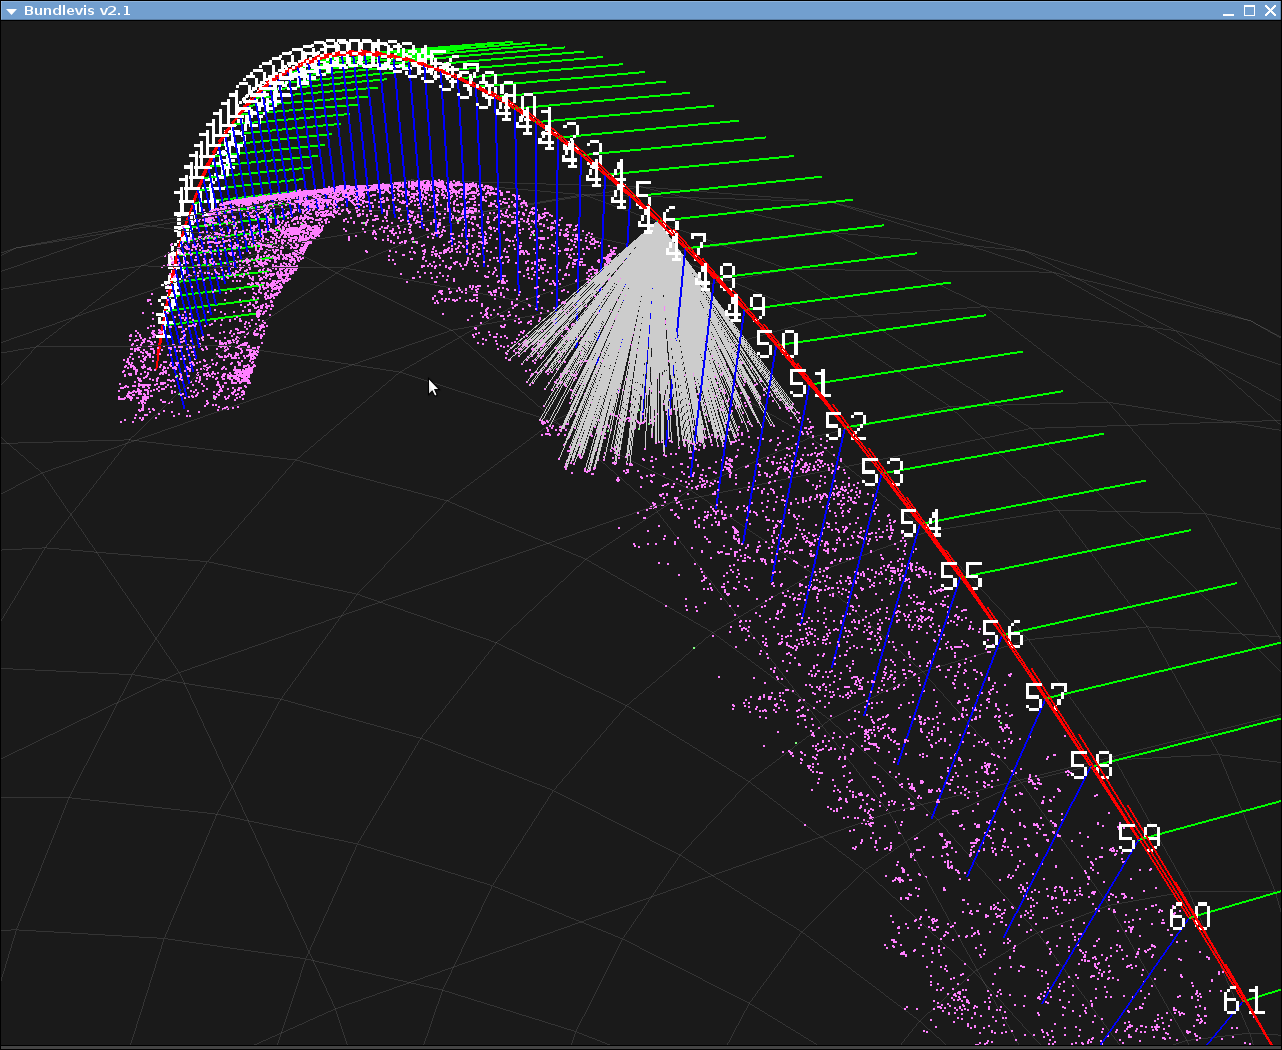
\includegraphics[width=6in]{images/bundlevis_apollo.png}
  \end{center}
  \caption{ A screenshot of bundle adjustment of Apollo 15's Orbit 33. }
  \label{fig:bundlevis}
\end{figure}

\begin{thebibliography}{1}

\bibitem{hartley04} Hartley, R.I. and Zisserman, A. ``Multiple View Geometry in Computer Vision,''
  Cambridge University Press. 2004. pp 597-627.
\bibitem{moore09} Moore, Wright, Schinstock, and Lewis. ``Comparison of Bundle Adjustment Formulations,''
  presented at ASPRS Annual Conf., Baltimore, Maryland, 2009.
\bibitem{triggs00} Triggs, McLauchlan, Hartley, and Fitzgibbon. ``Bundle Adjustment - A Modern Synthesis,''
  Lecture Notes in Computer Science. Vol. 1883, 298. January 2000

\end{thebibliography}
